\documentclass{article}

\usepackage{amsmath}
\usepackage{booktabs}  % nice tables
\usepackage[margin=25mm]{geometry}
\usepackage{natbib}
\usepackage{siunitx}  % use for all units
\usepackage{subcaption}  % for subfigures
\usepackage{todonotes}

\def\kph{\kilo\meter\per\hour}

\title{Bicycle Balance Assistance Reduces Probability of Falling at Low Speeds
When Subjected to Mechanical Perturbations}

\author{Marten T. Haitjema \and Leila Alizadehsaravi \and Jason K. Moore}

\begin{document}

\maketitle

\abstract{
  Uncontrolled bicycles are generally unstable at low speeds. We add a
  controlled steering motor to a consumer bicycle that stabilizes the bicycle
  at low speeds. To test the motor's assistance during falls, we apply varying
  magnitude external handlebar perturbations to the bicycle while ridden on a
  treadmill with the balance assist system activated and deactivated.  The
  probability of not recovering from a handlebar perturbation decreases when
  the balance assist is activated at a speed of 6~\si{\kph}.
}

\section{Introduction}
%
Single-actor bicycle crashes are associated with a suprisingly large number of
reported injuries~\citep{Wegman2024}. At low speeds, from start up to typical
cruising speeds, bicycles themselves are not self-stable and can be challenging
for the rider to balance. Low speed crashes may be reduced if the bicycle was
self-stable at these speeds, possibly relieving the rider of a necessary
control activity. Bicycles can be mechanically modified to lower the speeds at
which they are self-stable~\citep{Astrom2005} but since the 1980s it has been
known that applying a motor acutated steering torque proportional to the roll
rate can stabilize a single track vehicle at very low speeds. If this automatic
control of steering can stabilize a bicycle, it may reduce the control required
by the rider to successfully manage balancing tasks. We have developed such a
balance assisting bicycle and hypothesize that it helps the rider in situations
they are likely to fall.

Automatic roll stabilization of single track vehicles began in earnest after
predictive motorcycle models were developed and refined in throughout the
1970s. \Citet{vanZytveld1975} seems to be the first \todo{Check if a Japanese
researcher was first} to attempt to robotically stabilize a small motorbike
with a controlled inverted pendulum that mimicked rider lean, but he was not
successful in demonstrating what his theoretic control model correctly predicted. In his
model, he recognized that feedback of the vehicle roll angle and angular rate
was essential to stabilize the vehicle. It was not until the mid 1980s that
Ruijs and Pacjecka successfully demonstrated an automatically balanced
motorcycle~\citep{Ruijs1986} and they did so with a steering motor. Ruijs and
Pacejka clearly showed that steer torque driven by roll angle feedback
stabilizes the capsize mode, roll angular rate feedback stabilizes the weave
mode, and steer angular rate feedback stabilizes the wobble mode. They also
propose how the gains must change with respect to vehicle speed for
favorable control at all speeds. This roll motion feedback is the simplest
controller that can stabilize a single track vehicle above a minimum speed when
not concerned with wobble instabilities, which are not prominent in bicycles at
low speeds. Ruijs and Pacejka's work was not particularly concerned with low
speed stability and their vehicle was fully automatic, no human rider was
involved. Many more automatically balanced single track vehicles have been
demonstrated over the last 40 years, but none have demonstrated that increasing
low speed stability can assist in balancing and possibly reduce single actor
falls. Most of these robotic bicycles and motorcycles designers did not intend
for a human rider to also control the stabilized vehicle. Nevertheless, an
automatically stabilized bicycle can be controlled by a human rider if the
motor controlled steer torque and the rider applied steer torque act on the
steer in parallel. The effect of this automatic control gives the ability to
change the dynamics, up to some limits, of the human controlled plant.In our
prior study, we demonstrate reduced motion during
distractions~\cite{Alizadehsaravi2023} due to the balance assist but
researchers with a similar vehicle recently showed rider disatisfction with the
stabilization~\cite{Hanakam2023}.

The linear Carvallo-Whipple bicycle model~\citep{Carvallo1899,Whipple1899} is
the simplest bicycle model that exhibits non-minimum phase behavior and
self-stablity. Whipple even showed that roll motion feedback can stabilize the
system, remarkably in the early years of developments automatic control. The
bicycle model is ideal for showing the effect of a roll motion feedback driven
steer motor on the dynamics. The linear model can be described by the fourth
order state space equations:

\begin{align}
  \dot{\vec{x}} = \mathbf{A} \vec{x} +
  \mathbf{B}
  \vec{u}
  \textrm{ where }
  \vec{x} = \begin{bmatrix} \phi \\ \dot{\phi} \\ \delta \\ \dot{\delta} \end{bmatrix}
  \textrm{ and }
  \vec{u} = \begin{bmatrix} T_{\phi} \\ T_{\delta} \end{bmatrix}
\end{align}

The states are the roll angle \(\phi\) and steer angle \(\delta\) along with
their derivatives and the inputs are roll torque \(T_\phi\) and steer torque
\(T_\delta\). The state \(\mathbf{A}\) and input \(\mathbf{B}\) matrices are
functions of the equilbirum forward speed \(v\) and  are otherwise populated
with expressions that are functions of the geometric and inertial parameters of
the nonholonomic mulitbody system made up of four rigid bodies: two wheels,
front frame, and rear frame.

If the steer torque is the sum of the (h)uman applied torque and the (m)otor
applied torque \(T_\delta = T_\delta^\textrm{h} + T_\delta^\textrm{m}\),
\(\mathbf{B} = \begin{bmatrix} \mathbf{B}_\phi \quad \mathbf{B}_\delta
\end{bmatrix}\), and \(T_\delta^\textrm{m} = -k_{\dot{\phi}} \dot{\phi}\) then
the human controlled plant takes the form:

\begin{align}
  \dot{\vec{x}} = \left(\mathbf{A} -
  \mathbf{B}_\delta
  \left[0 \quad k_{\dot{\phi}} \quad 0 \quad 0\right]
\right)
  \vec{x} + \mathbf{B} \begin{bmatrix} T_{\phi} \\ T_\delta^\textrm{h} \end{bmatrix}
\end{align}

The state matrix \(\mathbf{A}\) and input matrix \(\mathbf{B}\) are both
functions of the equilibrium speed \(v\) and \(k_{\dot{\phi}}\) can be selected
such that the eigenvalues of \(\left(\mathbf{A} - \mathbf{B}_\delta\left[0 \quad k_{\dot{\phi}}
\quad 0 \quad 0\right] \right)\) have negative real parts for
\(v_{weave} < v < v_{capsize}\). With gain scheduling with respect to \(v\),
the speed range where the bicycle is stable can be maximized within
any physical acutator magnitude and bandwidth limits. \citet{Schwab2008}
elaborates on some of the possibilities in scheduling the gains for such a
controller on this model.

\todo[inline]{I'm not consistent with the arrow being a vector for $B_\delta$}

In this paper, we test whether a gain scheduled steer motor controlled bicycle
that is stable at a low speed range when riderless assists in balancing by
investigating whether it is beneficial in preventing the rider from falling.
To do this, we apply varying magnitude mechanical perturbations to the
handlebars while the rider is balancing the bicycle on a treadmill and then
assess the rider's probability of falling with the balance assist steer motor
system on and off.

\section{Methods}
%
\subsection{Bicycle}
%
We modified a standard electric bicycle (Gazelle Grenoble C7, Dieren, The
Netherlands) with a custom motor in the steering assembly capable of applying
up to 7~\si{\newton\meter} of torque between the head tube and steer tube. A
custom motor controller converts the commanded torque to applied torque. We
measure the speed of the rear wheel with an encoder (Magura XXX) and measure
the body fixed roll rate of the bicycle with a MEMs rate gyroscope (Company,
Location).  The balance assist control algorithm is implemented on a
microprocessor (Teensy, Company, Location) and data from all sensors is logged
with a CAN bus (Company, Location) at approximately X Hz.

\subsection{Balance Assist Control}
We use a forward speed \(v\) gain scheduled proportional roll rate feedback
controller to stabilize the bicycle. The commanded steer torque
\(T^\textrm{m}_\delta\) from the steer motor follows the control law
\begin{align}
  T^\textrm{m}_\delta = k(v_{weave} - v)\dot{\phi}
\end{align}
where 4.7~\si{\meter\per\second} is the weave critical speed predicted from the
open loop bicycle rigid-rider dynamics. We use \(k=8\) and \(k=10\) as gain
values during the experiments. Scaling the proportional feedback gain linearly
with respect to speed stabilizes the normally unstable weave mode of the
bicycle from speeds of X~\si{\kilo\meter\per\hour} to
X~\si{\kilo\meter\per\hour} as shown in Figure~\ref{fig:eigenvalues}.

\begin{figure}
  \centering
  \subcaptionbox{}{
    \includegraphics[width=3in]{figures/uncontrolled-eig-vs-speeds.png}
  }
  \subcaptionbox{}{
    \includegraphics[width=3in]{figures/balance-assist-controllers-eig-vs-speeds.png}
  }
  \caption{Uncontrolled (a) and controlled (b) root locus of eigenvalue
    components (real: solid, imaginary: dashed) plotted versus speed. Vertical
    blue lines indicate the two speeds we perform experiments at. Green shaded
    region is the linear stable range.}
  \label{fig:eigenvalues}
\end{figure}

\todo[inline]{Decide on what physical parameters to use.}

\subsection{Perturbations}
%
We apply external longitudinal forces to the ends of each handlebar using an
adapted Bump'Em system~\cite{Tan2020} which is designed with four motors
working in tandem. The four motors are programmed to apply a light force at all
times to keep the ropes taught and to track a commanded force profile using a
PID controller running on a microprocessor (Arduino XXX, Italy). We measure the
force applied by each motor at the handlebar via four inline load cells, each
with a max load of XX~\si{\newton}. The commanded force profiles are designed
to apply an external pulsive torque to the front assembly (handlebars, forks,
wheel) at magnitudes varying from X to X. The four motors are arranged at the
four corners of a 1~\si{\meter} wide treadmill (make, Company, City) that can
reach speeds of 18~\si{\kilo\meter\per\hour}. The general design is described
in detail in the Van De Velde's MSc thesis~\cite{vandeVelde2022a}. Our
modifications relative to that described in the thesis include simplifying the
controller with a inexpensive microcontroller and the use of a simpler safety
harness.

\begin{figure}
  \centering
  % TODO : scale these pngs to a reasonable size for an A4 sheet
  \subcaptionbox{}{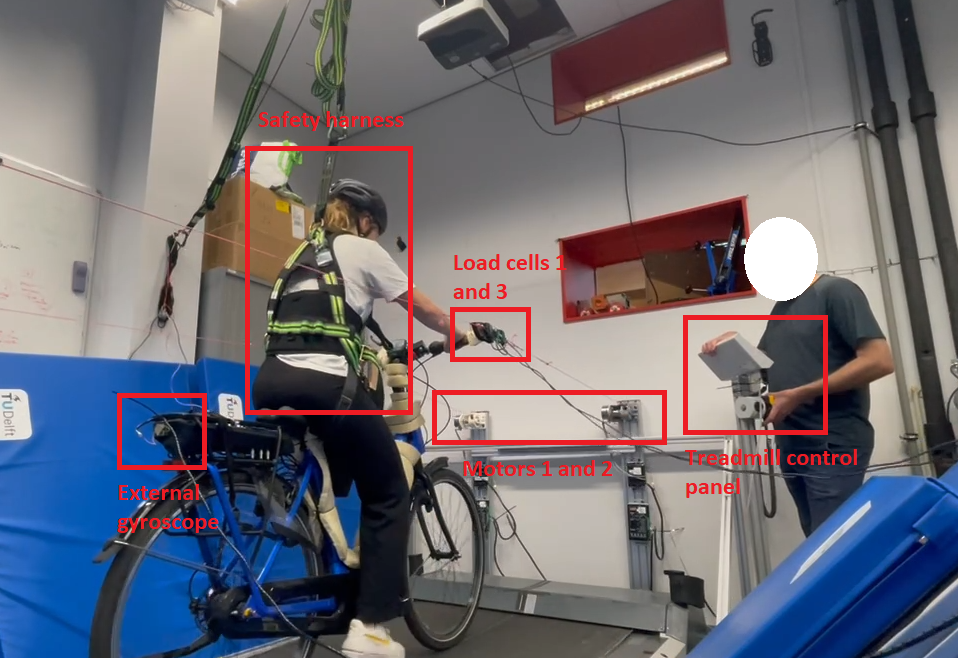
\includegraphics[width=70mm]{figures/participant-in-set-up.png}}
  \subcaptionbox{Diagram of perturbation system.}{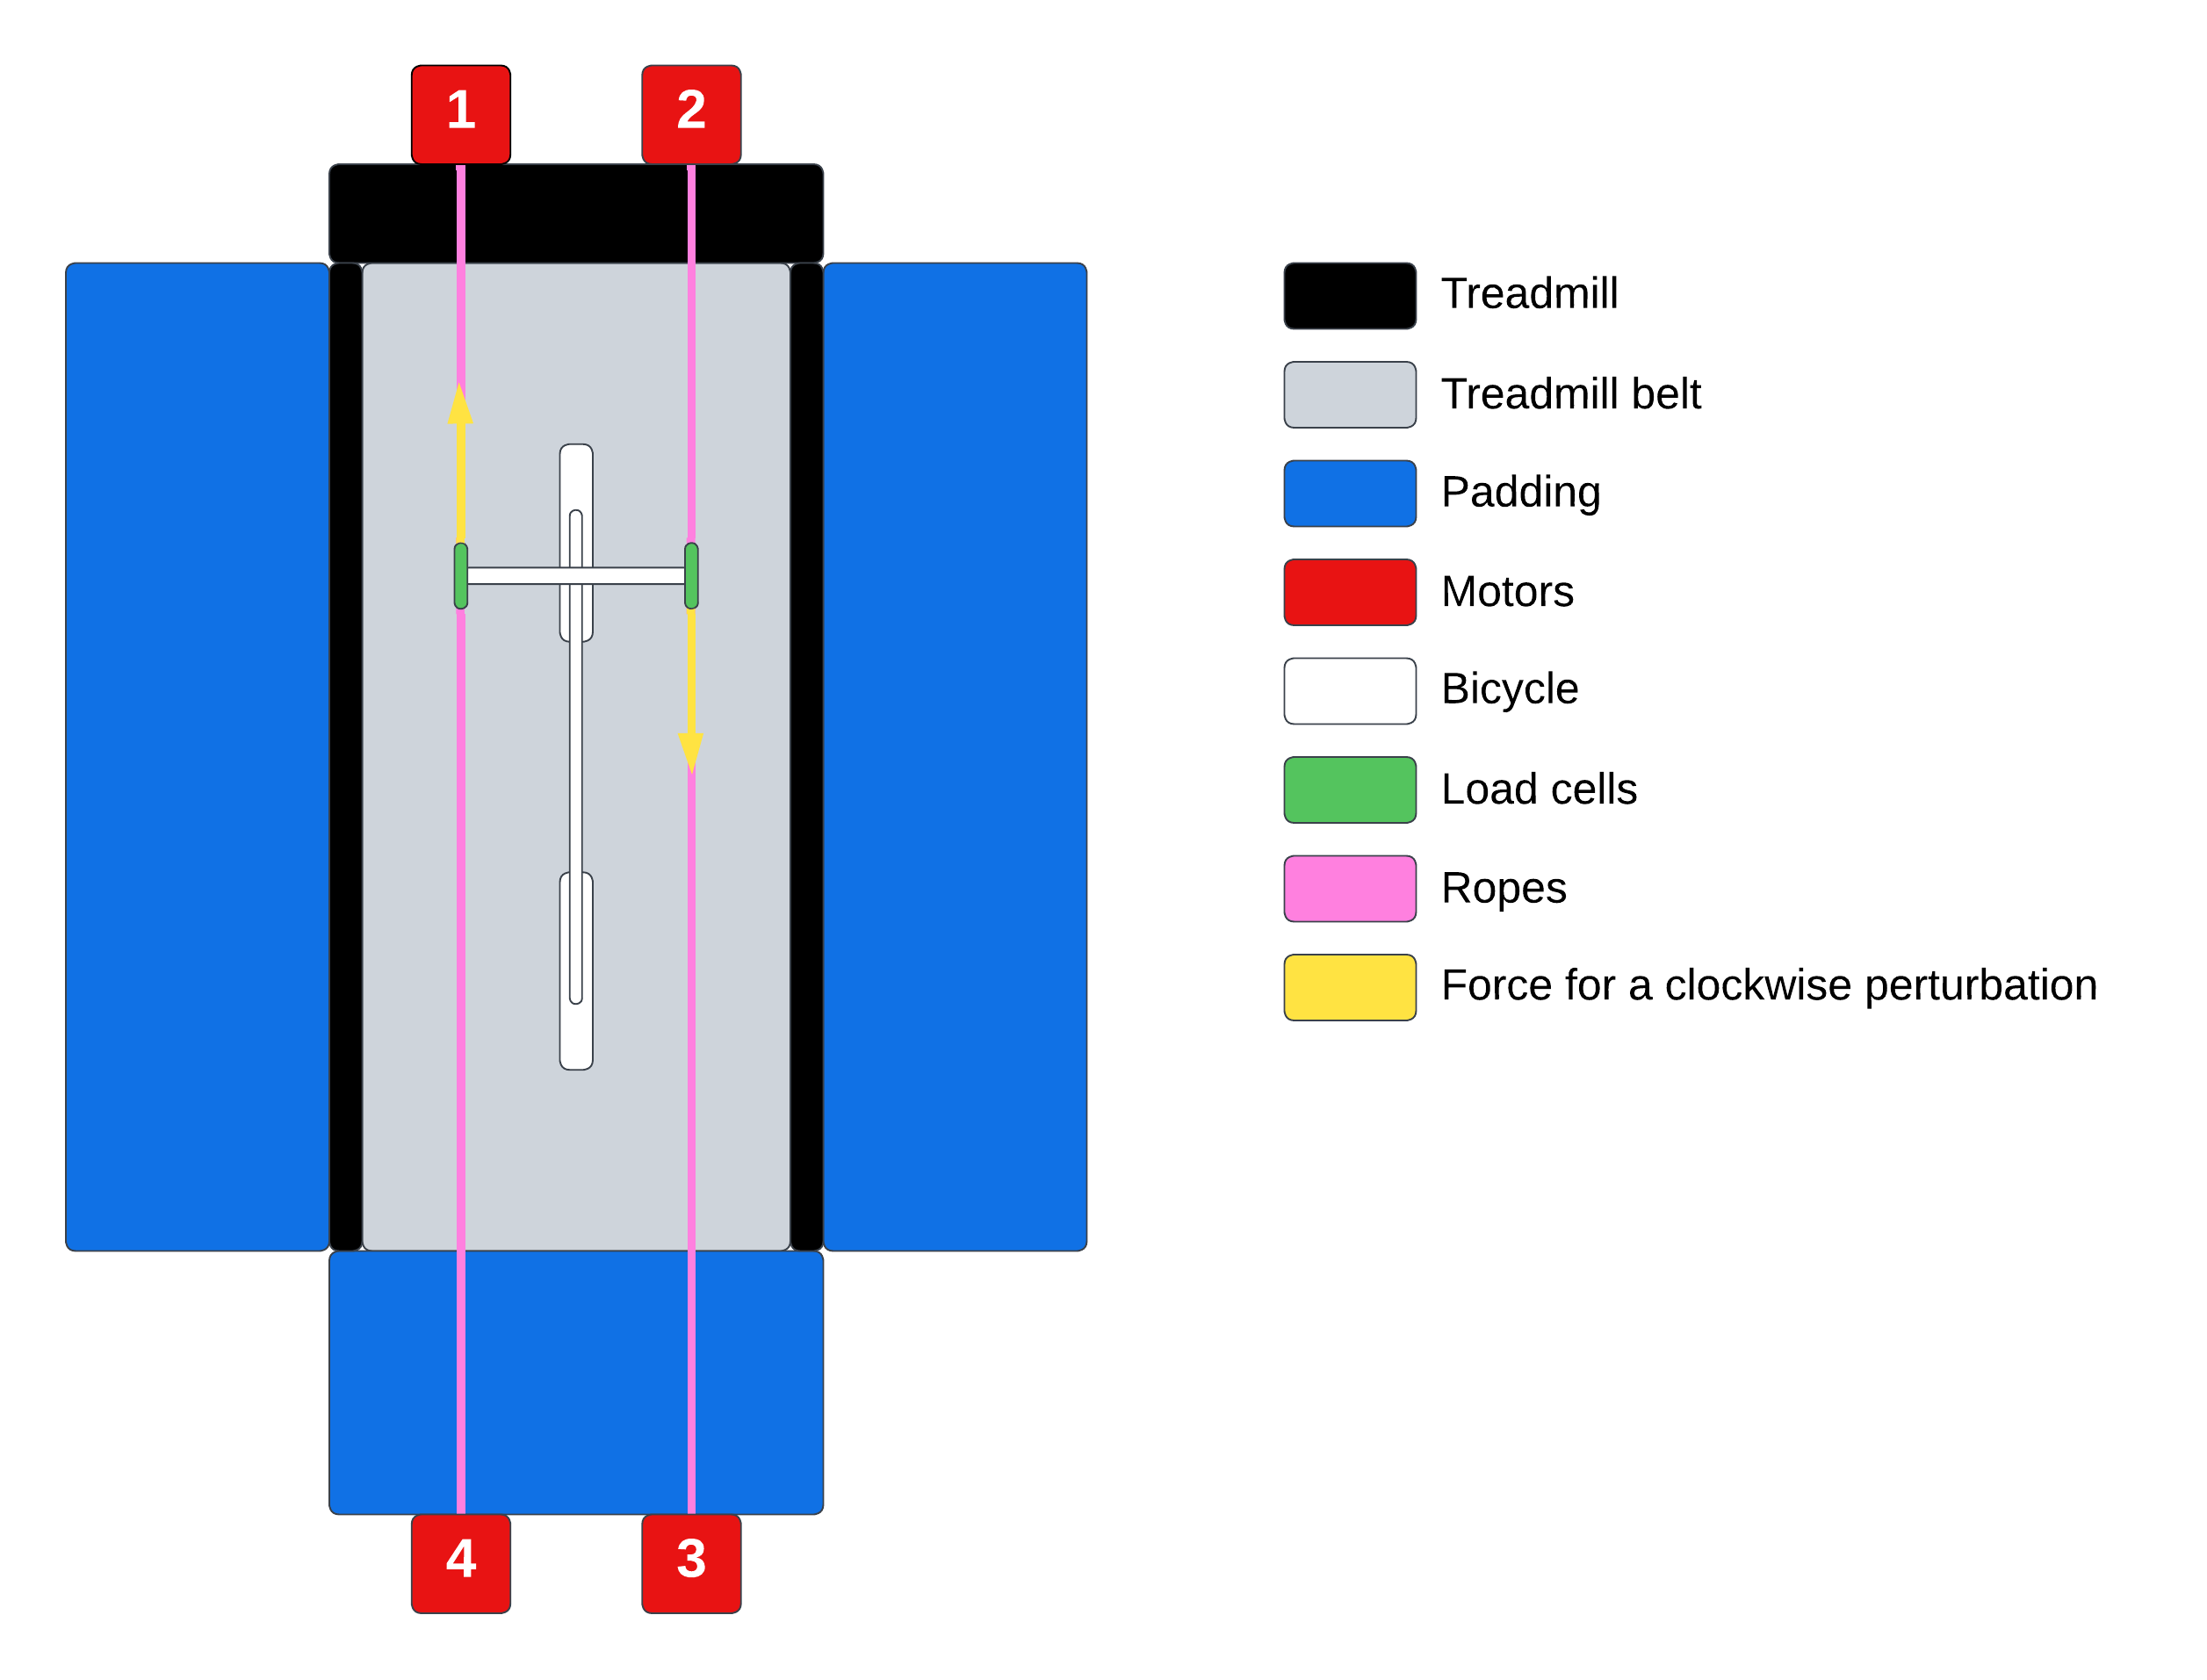
\includegraphics[width=70mm]{figures/setup-diagram.png}
}
\end{figure}

\begin{figure}
  \includegraphics{example-image-a}
  \caption{Force nd torque plts of a pterubation of 80N per rope in the
  counterclockwise direction (from Marten's thesis, pg 26)}
\end{figure}

\begin{figure}
  \centering
  \subcaptionbox{Start}{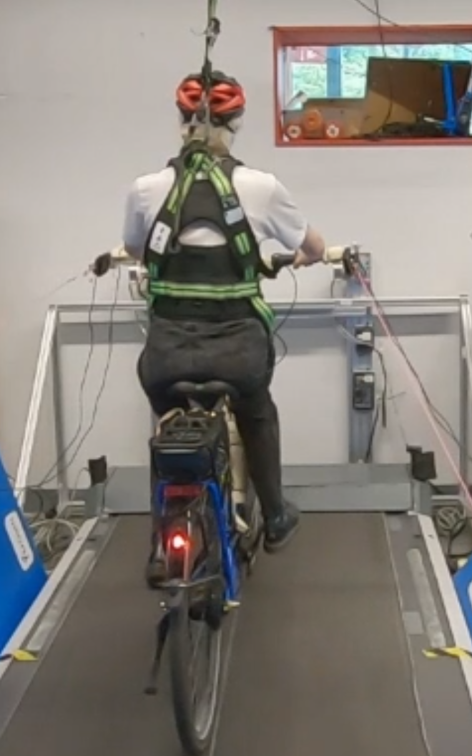
\includegraphics[width=60mm]{figures/start.png}}
  \subcaptionbox{During}{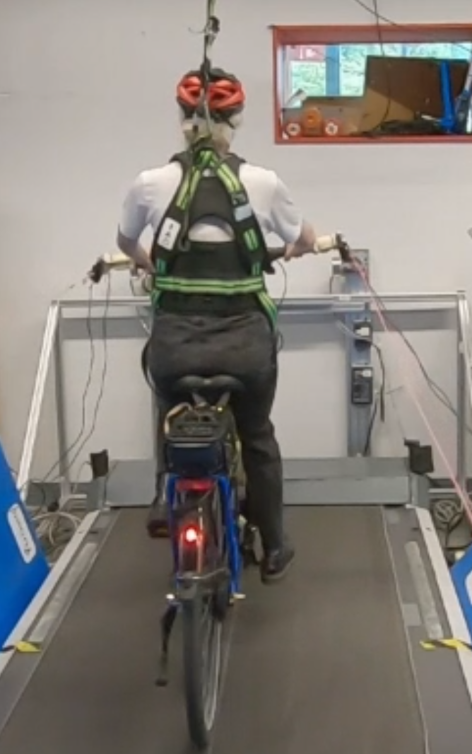
\includegraphics[width=60mm]{figures/during.png}}
  \subcaptionbox{After}{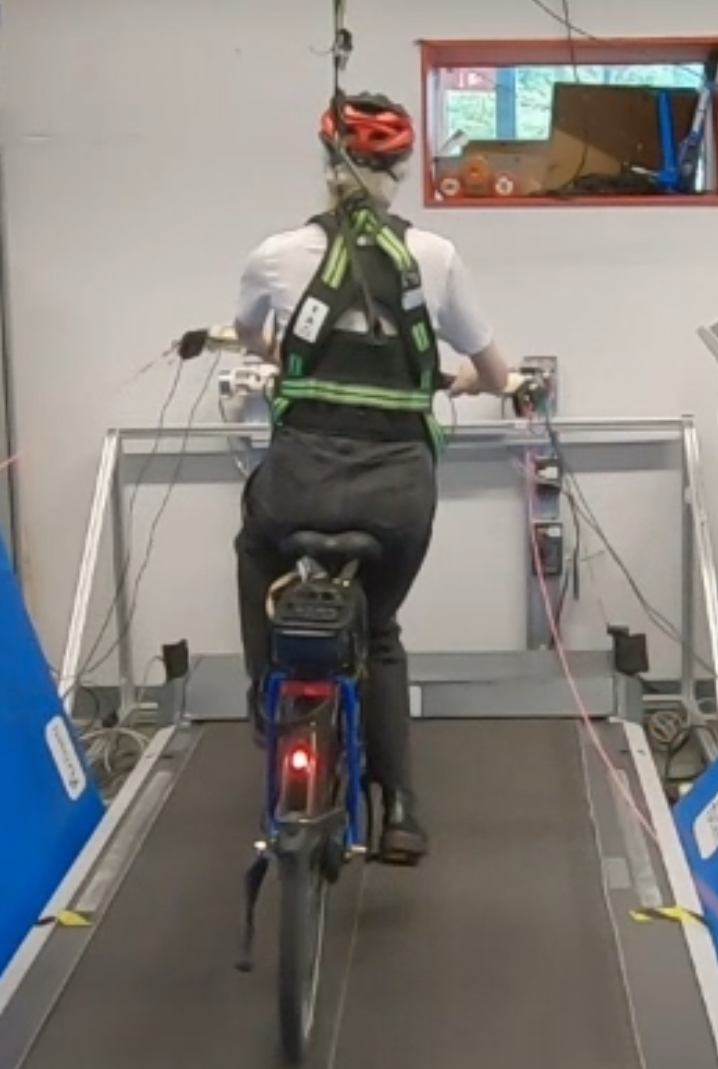
\includegraphics[width=60mm]{figures/after.png}}
  \subcaptionbox{Recovery}{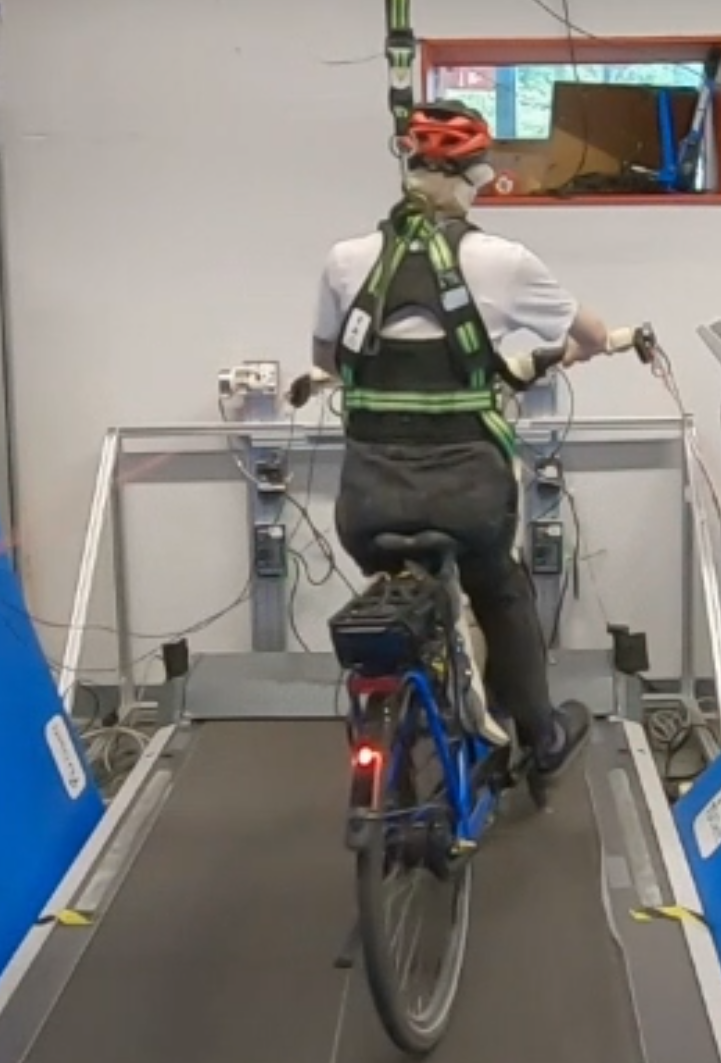
\includegraphics[width=60mm]{figures/recovery.png}}
  \caption{Thesis Fig 5.1 on pg 37}
\end{figure}

\subsection{Subjects}
%
We recruited 26 able-bodied young adults (20-36 years old) to participate in
the experiments. The subjects all were confident in their cycling skills and
had cycled at least once in the last month. Eleven subjects performed the
experiments at 1.7~\si{\meter\per\second} (6~\si{\kilo\meter\per\hour}) and
fifteen subjects performed the experiments at 2.8~\si{\meter\per\second}
(10~\si{\kilo\meter\per\hour}). All subjects consented to the experiment and
could decline to continue at any time. The study was approved by Delft
University of Technology's Human Research Ethics Council (\#XXX).

\subsection{Protocol}
%
The subjects were divided into two groups. Tthe first group performed the
protocol at a belt speed of 10~\si{\kph} with the controller gain as $k=8$ and
the second group performed the protocol at a belt speed of 6~\si{\kph}. The
10~\si{\kph} group's experiments occured X weeks before the
6~\si{\kilo\meter\per\hour} group.

Subjects wore a helmet and fall safety harness attached to the ceiling. We
allowed them practice riding on the treadmill until they indicated they were
comfortable enough to have perturbations applied. For most, this was less than a
10~\si{\minute} warm up. We then asked the rider to ride for 90~\si{\second},
attempting to maintain the location of their front wheel on the center line of
the treadmill. We define a ``fall'' on the treadmill by two criteria: the rider
removes their foot from the pedal and places it on the ground or the bicycle
wheel exceeds the width of the treadmill. We then applied perturbations in
random directions (clockwise or counter clockwise) increasing the magnitude by
X~\si{\newton\meter} each time. We log the magnitude that causes the first fall
to characterize that subject's nominal fall threshold. Following this we apply
20 perturbations of random magnitudes to the cyclist while they ride at a
constant speed and record which perturbations cause a fall. We let the cyclist
rest and then perform another 20 perturbations. We randomize whether the
balance assist system is on or off during the first or second set of
perturbations.

Following the initial threshold determination, we choose perturbation forces
according to a random and adaptive staircase procedure applying
perturbations above and below the initial perturbation threshold, while
allowing small progression of the perturbation threshold to accommodate
learning effects. The goal of this adaptive staircase procedure is to have
participants fall for approximately 50\% of the time. The procedure
consists of twenty perturbations per condition. Participants undergo two
conditions: twenty perturbations with the balance-assist turned on and twenty
perturbations with the balance-assist turned off (in randomized order).

Five possible perturbation forces are determined based on the initial
perturbation threshold estimate: the initial estimate itself, two perturbations
lower than the initial estimate and two perturbations higher than the initial
estimate.  The five possible perturbations are separated by 10 N steps. For
example, if the initial estimate of the perturbation threshold of a participant
is 80 N, the five possible perturbations are 60, 70, 80, 90 and 100 N. Which
one of these five perturbations is chosen is determined at random. If the
perturbation results in a fall, the estimate of the perturbation threshold is
decreased with 10 N, and vice versa if the perturbation did not result in a
fall. Five new possible perturbation forces are determined around the updated
perturbation threshold, and a new perturbation is selected at random. This
process iterates until twenty perturbations are applied.

\subsection{Measurements}
%
We measure the time histories of the Bump'Em delivered perturbation forces and
the bicycle's steer angle, roll angle, roll angular rate, and forward speed.
%
\begin{table}
  \caption{Raw measurements}
  \begin{tabular}{llll}
    \toprule
    Measure & Variable & Units & Sensor \\
    \midrule
    Perturbation Order Number & \(j\) & integer & NA\\
    Perturbation Force \(l\)eft/\(r\)ight,\(f\)ront/\(r\)ear & \(F_{lf},F_{rf},F_{lr},F_{rr}\) & \si{\newton} & Load cell\\
    Steer Angle & \(\delta\) & \si{\degree} & encoder \\
    Roll Angle & \(\phi\) &  \si{\degree} & Kalman estimate \\
    Roll Angular Rate & \(\dot{\phi}\) &  \si{\degree\per\second} & rate gyroscope \\
    Balance Assist Gain & \(k\) & TODO & NA \\
    Bicycle Speed & \(v\) & Meters per second & wheel encoder \\
    \bottomrule
  \end{tabular}
\end{table}

Based on the findings in \cite{Haitjema2023a}, we calculate several variables.
We use the angular impulse \(L\) due to the perturbation forces over a
0.3~\si{\second} duration to characterize the magnitude of delivered
perturbation. The duration is selected based on the duration of the commanded
force.

\begin{align}
  F_r = & F_{rf} - F_{rr} \\
  F_l = & F_{lf} - F_{lr} \\
  L = & \int_{0\si{\second}}^{0.3\si{\second}} l/2(F_r + F_l) dt
\end{align}

We characterize the skill of the rider by calculating the standard deviation of
the steer angle \(\sigma_\delta\) over the 90~\si{\second} period they were
asked to maintain their position at the center of the treadmill. At the
initiation of each perturbation we log the steer and roll angles to characterize
the configuration of the bicycle when perturbed. The gain setting on the
balance assist controller indicates if the assistance is off \(k=0\) or on at
two different levels: low \(k=8\) or high \(k=10\). A recovery from the
perturbation is successful if the person neither put their foot down onto the
treadmill surface or either wheel of the bicycle exits the width of the
treadmill belt. We record this as a binary variable \(f\).

\begin{figure}
  \centering
  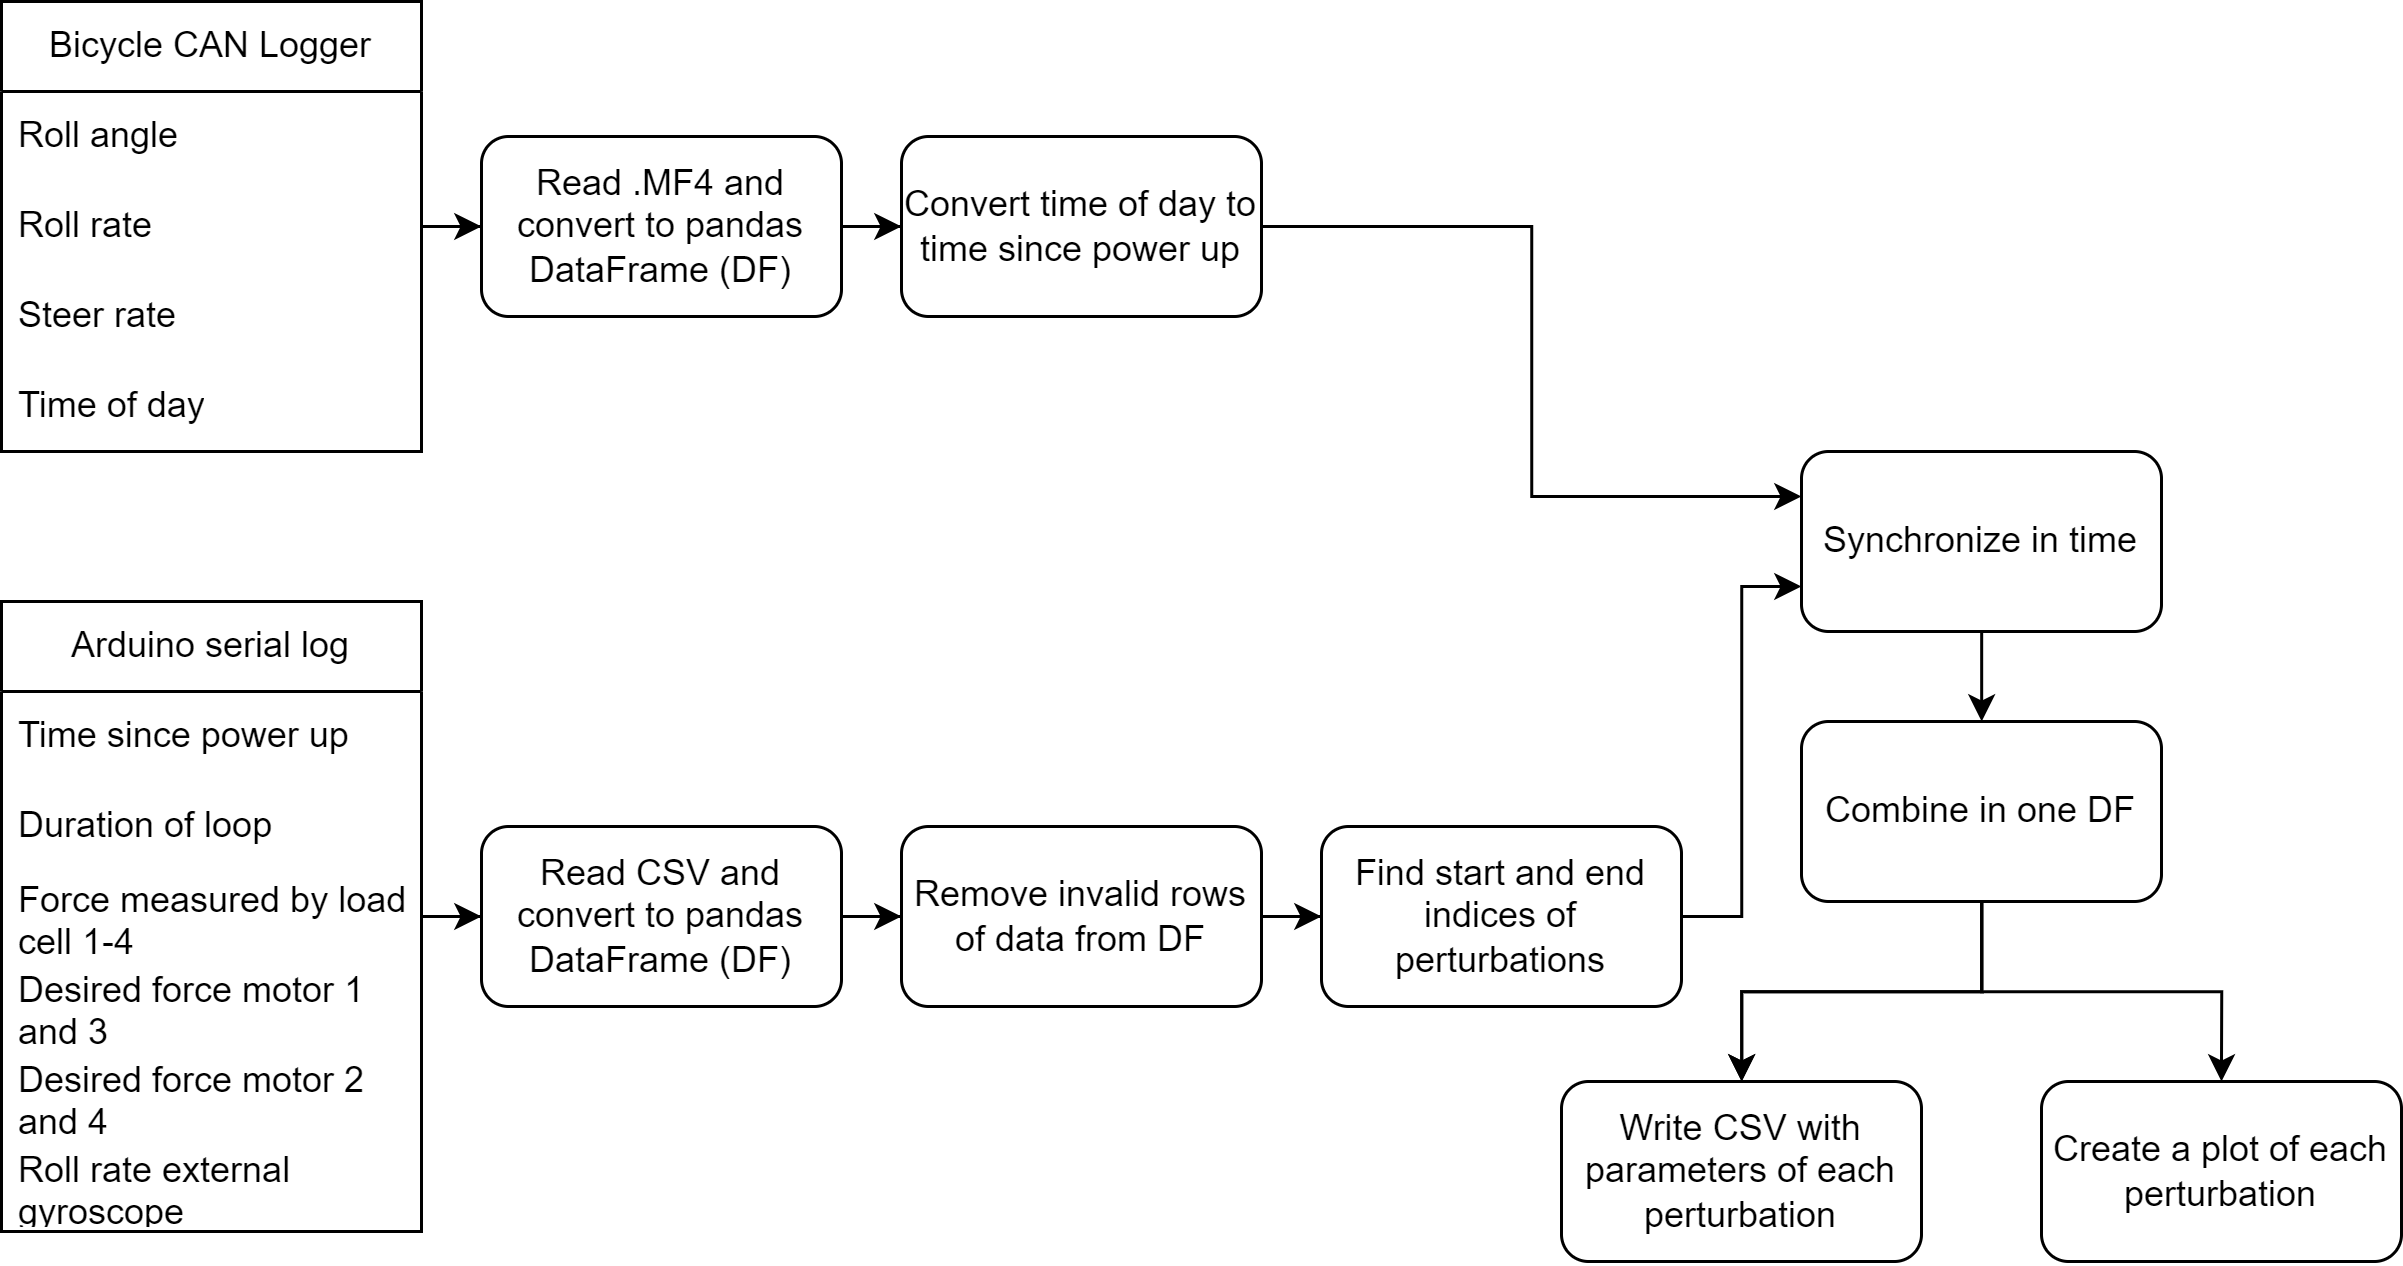
\includegraphics[width=\columnwidth]{figures/data-processing.png}
  \caption{Thesis Fig 3.13 on pg 27}
\end{figure}

\subsection{Statistics}
%
We test the hypothesis that the balance assistance controller will reduce the
probability of falling when perturbed externally at the handlebar. We have a
single binary outcome variable \(f\) that is dependent on several possible
explanatory independent variables including the binary balance assistance (on
or off).

\begin{table}
  \begin{tabular}{lll}
    \(L\) & \si{\newton\meter\second} & angular impulse of the applied
    perturbation torque \\
    \(c\) & integer & order number of perturbation \\
    \(\sigma_\delta\) & standard deviation of steer angle during Phase X \\
    \(k\) & TODO & gain of balance assist control \\
    \(\delta_0\) & \si{\degree} & steer angle at start of perturbation \\
    \(\phi_0\) & \si{\degree} & roll angle at start of perturbation \\
    \(v\) & \si{\meter\per\second} & forward speed (6 or 10) \\
    \(f\) & boolean & outcome of perturbation: did not fall, did fall \\
  \end{tabular}
\end{table}

We evaluate this hypothesis using a multivariate logistic regression model.

\begin{align}
  f_{ij} | p_{ij} \sim \textrm{Bern}(p_{ij})
\end{align}

\(f_{ij}\) is the binary outcome of perturbation \(j\) of participant \(i\)
which follows a Bernoulli distribution given the probability \(p_{ij}\) that a
fall occurs. The log-odds of the probabiliy is then a linear function of our
independent variables with \(\beta\) as the intercept and \(\alpha_k\) as the
linear coefficients.

\begin{align}
  \log \left(\frac{p_{ij}}{1-p_{ij}} \right) = \beta + \sum_{k=0}^{K} \alpha_k x_{ij}^{k}
\end{align}

\todo[inline]{we already use k for gain}

We scalle all independent variables such they they have a mean of zero and a
standard deviation of one. We use cluster-mean centering, as recommended by
\cite{Enders2007}, with the clusters being an individual subject because we are
interested in the association between the state of the balance-assist system
and the outcome of the perturbation.

Cluster-mean centering shows there to be no variation between participants,
i.e. that rider skill (the only participant differentiating factor) is not a
predictor. We expected there to be a variation between participants in how well
they are able to resist the perturbation. However, this was not true. This
allowed us to use a simpler single-level logistic regression model, instead of
a multilevel model. This left use with angular impulse, perturbation order,
balance assist state, and roll \& steer angles at the time of perturbation. We
also include interaction effects between the balance assist state and the other
four variables.

\todo[inline]{Marten writes ``The skill variable is not included, because it
was not collected correctly for all participants.'' This needs to be addressed.
What about skill being tied to participant clusters?}

We divide the analysis into two separate model evalautions, one for the
6~\si{\kilo\meter\per\hour} \(k=10\) trials and one for the
10~\si{\kilo\meter\per\hour} \(k=8\) trials and we evaluate our hypothesis for
each set of data.

\section{Results}

The coefficient estimates for a single-level logistic regression at
6~\unit{\kilo\meter\per\hour} with gain $k=10$ are shown in Table
\ref{table:freq-coefs-6}. The angular impulse, perturbation order, and balance
assist state are all statistically significant predictors. Larger angular
impulse increases the probability to fall and enduring more perturbations or
having the balance assist on, decrease the probability to fall.  The associated
multiplicative change in odds are shown in
Table~\ref{table:freq-change-in-odds-6}.

\begin{table}
  \centering
  \caption{Logistic regression coefficient estimates at
    6~\unit{\kilo\meter\per\hour} and gain $k=10$.}
  \label{table:freq-coefs-6}
  \begin{tabular}{lrrr}
    \toprule
    Variable                                      & Estimate          & Standard error          & p-value          \\
    \midrule
    Intercept                                     & -0.29             & 0.17                    & 0.09             \\
    Angular impulse                               & 1.69              & 0.27                    & 0.00             \\
    Perturbation order                            & -0.77             & 0.22                    & 0.00             \\
    Balance assist state                          & -0.64             & 0.27                    & 0.02             \\
    Roll angle                                    & -0.25             & 0.21                    & 0.24             \\
    Steer angle                                   & -0.14             & 0.21                    & 0.51             \\
    Balance-assist on $\times$ roll angle         & 0.52              & 0.34                    & 0.12             \\
    Balance-assist on $\times$ steer angle        & -0.41             & 0.34                    & 0.22             \\
    Balance-assist on $\times$ angular impulse    & 0.41              & 0.41                    & 0.32             \\
    Balance-assist on $\times$ perturbation order & -0.53             & 0.34                    & 0.12             \\
    \bottomrule
  \end{tabular}
\end{table}

\todo[inline]{Combine the columns of the multiplicative change in odds into the
coefficient table}

\begin{table}
  \centering
  \caption{Multiplicative change in odds of predictor variables at 6
  \unit{\kilo\meter\per\hour} and gain $k=10$ based on frequentist
         single-level logistic regression.}
  \label{table:freq-change-in-odds-6}
  \begin{tabular}{lllll}
      \textbf{Variable}                             & \textbf{Multiplicative change in odds} & \textbf{2.5\%} & \textbf{97.5\%} & \textbf{p-value} \\ \hline
      Intercept                                     & 0.75                                   & 0.53           & 1.05            & 0.09             \\
      Angular impulse                               & 5.40                                   & 3.18           & 9.16            & 0.00             \\
      Perturbation order                            & 0.46                                   & 0.30           & 0.72            & 0.00             \\
      Balance-assist on                             & 0.53                                   & 0.31           & 0.89            & 0.02             \\
      Roll angle                                    & 0.78                                   & 0.51           & 1.18            & 0.24             \\
      Steer angle                                   & 0.87                                   & 0.58           & 1.32            & 0.51             \\
      Balance-assist on $\times$ roll angle         & 1.68                                   & 0.86           & 3.29            & 0.12             \\
      Balance-assist on $\times$ steer angle        & 0.66                                   & 0.34           & 1.28            & 0.22             \\
      Balance-assist on $\times$ angular impulse    & 1.51                                   & 0.67           & 3.38            & 0.32             \\
      Balance-assist on $\times$ perturbation order & 0.59                                   & 0.30           & 1.15            & 0.12             \\
  \end{tabular}
\end{table}

The coefficient estimates for a single-level logistic regression at
10~\si{\kilo\meter\per\hour} with gain $k=8$ are shown in Table
\ref{table:freq-coefs}. The angular impulse and perturbation order are
statistically significant predictors. Larger angular impulse increases the
probability to fall and enduring more perturbations decreases the probability
to fall. The associated multiplicative change in odds are shown in
Table~\ref{table:freq-change-in-odds}.

\begin{table}
  \centering
  \caption{Logistic regression coefficient estimates at
    10~\unit{\kilo\meter\per\hour} and gain $k=8$.}
  \label{table:freq-coefs}
  \begin{tabular}{lrrr}
    \toprule
    Variable                                      & Estimate          & Standard error          & p-value \\
    \midrule
    Intercept                                     & -0.24             & 0.16                    & 0.13    \\
    Angular impulse                               & 2.39              & 0.29                    & 0.00    \\
    Perturbation order                            & -1.16             & 0.21                    & 0.00    \\
    Balance-assist on                             & -0.44             & 0.24                    & 0.07    \\
    Roll angle                                    & 0.27              & 0.22                    & 0.22    \\
    Steer angle                                   & -0.37             & 0.24                    & 0.12    \\
    Balance-assist on $\times$ roll angle         & -0.61             & 0.34                    & 0.08    \\
    Balance-assist on $\times$ steer angle        & 0.56              & 0.35                    & 0.11    \\
    Balance-assist on $\times$ angular impulse    & 0.46              & 0.44                    & 0.29    \\
    Balance-assist on $\times$ perturbation order & -0.37             & 0.32                    & 0.25    \\
    \bottomrule
  \end{tabular}
\end{table}

\begin{table}
  \centering
  \caption{Multiplicative change in odds of predictor variables at 10 \unit{\kilo\meter\per\hour} based on
      frequentist single-level logistic regression.} \label{table:freq-change-in-odds}
  \begin{tabular}{lllll}
    \textbf{Variable}                             & \textbf{Multiplicative change in odds} & \textbf{2.5\%} & \textbf{97.5\%} & \textbf{p-value} \\ \hline
    Intercept                                     & 0.78                                   & 0.57           & 1.07            & 0.12             \\
    Angular impulse                               & 10.92                                  & 6.23           & 19.13           & 0.00             \\
    Perturbation order                            & 0.31                                   & 0.21           & 0.48            & 0.00             \\
    Balance-assist on                             & 0.64                                   & 0.40           & 1.03            & 0.07             \\
    Roll angle                                    & 1.31                                   & 0.85           & 2.04            & 0.22             \\
    Steer angle                                   & 0.69                                   & 0.43           & 1.10            & 0.12             \\
    Balance-assist on $\times$ roll angle         & 0.54                                   & 0.28           & 1.07            & 0.08             \\
    Balance-assist on $\times$ steer angle        & 1.76                                   & 0.88           & 3.50            & 0.11             \\
    Balance-assist on $\times$ angular impulse    & 1.59                                   & 0.68           & 3.74            & 0.29             \\
    Balance-assist on $\times$ perturbation order & 0.69                                   & 0.37           & 1.30            & 0.25             \\
  \end{tabular}
\end{table}

\begin{figure}
  \includegraphics{example-image-a}
  \caption{Box plot or distrubtion plot showing graphical view of stats
  tables.}
\end{figure}

\section{Discussion}

\subsection{Balance-assist}

Turning the balance-assist system on significantly \((p<0.05)\) reduces the
odds that a fall occurs while cycling at a speed of 6~\si{\kph} but at
10~\si{\kph} that is not the case \((p=0.07)\). If all other factors remain the
same at 6~\si{\kph}, the balance-assist system halves the odds that a
perturbation results in a fall. How much this changes the probability that a
fall occurs depends on the values of the other predictor variables: if the odds
that a perturbation results in a fall are a 1000:1, turning on the
balance-assist system reduces the odds to 500:1. However, the probability that
a fall occurs is only reduced from $0.999$ to $0.998$. On the other hand, if
the odds that a fall will occur are smaller, halving the odds has a larger
influence on the fall probability. For example, if the odds that a fall occurs
is two, halving it to one reduces the probability from $0.66$ to $0.50$. Figure
\ref{fig:probability} shows how the balance-assist system changes the fall
probability for different magnitudes of angular impulse.

\begin{figure}
  \centering
  \subcaptionbox{6~\si{\kph}}{
  \includegraphics[width=70mm]{example-image-a}
    %\includegraphics[width=\textwidth]{figures/predicted_fall_probability-6.png}
  }
  \subcaptionbox{10~\si{\kph}}{
    \includegraphics[width=70mm]{example-image-b}
  }
  \caption{Comparison of predicted fall probability for balance-assist on or
    off All other predictor variables are fixed at zero, except for the
    interaction effect between the balance-assist and the angular impulse.}
  \label{fig:probability}
\end{figure}

Angular impulse magnitude has the largest significant effect for predicting
fall probability. An increase in angular impulse increases the fall probability
both at 6 and 10~\si{\kph}. At 10~\si{\kph}, the multiplicative change in odds
is approximately twice as big as at 6~\si{\kph}. Thus, angular impulse is a
more important predictor at higher speeds compared to lower speeds. The reason
for this likely has to do with the width of the treadmill. As a bicycle travels
at higher speeds, the same perturbation causes larger lateral deviations. At
10~\si{\kph} almost all falls were due to the bicycle exiting the maximum width
of the treadmill. If the same experiment was performed on an infinite plane,
the riders may have recovered from the perturbation. At 6~\si{\kph} the riders
could often recover in the alloted treadmill width. Our results are very much
dependent on the two modes of falling with use: exit the treadmill width or
foot is placed on the belt. Cycle paths are a similar width as the treadmill,
so ride's are often limited in width when recoverying from a fall.

\todo[inline]{Could show an impulse response in lateral deviation for different
speeds.}

An increase in the number of perturbation that a participant already
experienced, decreases the probability that a fall occurs. This is likely due
to the participants learning how to better recover from the perturbation over
the duration of the experiment. This effect is significant at both 6 and
10~\si{\kph}, and in the same order of magnitude. This suggests that the
learning effect that occurs during the experiment is not strongly dependent on
the speed.

Roll and steer angle are not a significant predictor of fall probability,
neither at 6 or at 10~\si{\kph}. We expected this to have an effect. If you are
in a rolled and steered state that is far from the upright equilibrium, then a
perturbation that further pushes you from the equilibrium should have some
additive or multiplicative effect on the resulting motion trajectory.

None of the interaction effects are statistically significant. That means that
whether the balance-assist system is on or off does not significantly change
the effect that the roll angle, steer angle, angular impulse, and perturbation
order have on the probability that a fall will occur.

\section{Conclusion}

\bibliographystyle{apalike}
% NOTE : this file is automatically generated from Zotero, do not edit
% manually!
\bibliography{references}

\end{document}
